\documentclass{article}
\usepackage[left=0.05in, right=0.05in, top=0.05in, bottom=0.05in]{geometry}
% \usepackage{fullpage}
\usepackage{graphicx}
\usepackage{subfigure}

\begin{document}
	\begin{center}
		\Huge Uniform node interpolation
	\end{center}
	\begin{figure}[!htbp]
		\begin{center}
		\subfigure[$5$ nodes]{
			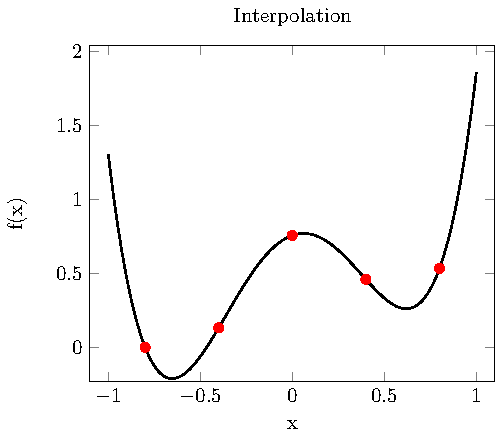
\includegraphics[width=0.4\textwidth]{./Uniform_5.pdf}
		}
		\subfigure[$10$ nodes]{
			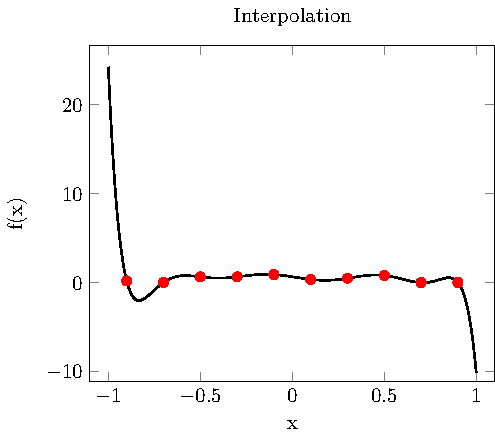
\includegraphics[width=0.4\textwidth]{./Uniform_10.pdf}
		}

		\subfigure[$20$ nodes]{
			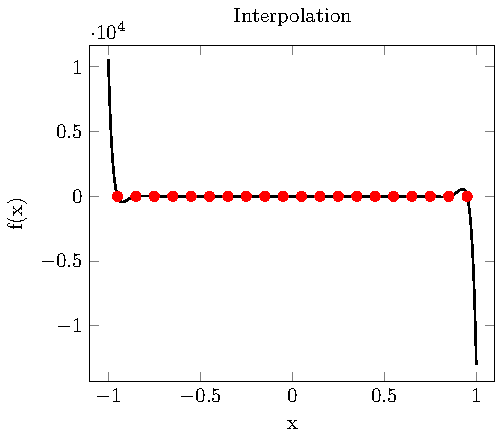
\includegraphics[width=0.4\textwidth]{./Uniform_20.pdf}
		}
		\subfigure[$50$ nodes]{
			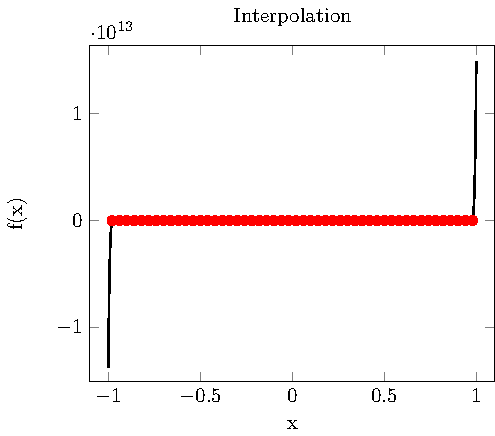
\includegraphics[width=0.4\textwidth]{./Uniform_50.pdf}
		}

		\subfigure[$100$ nodes]{
			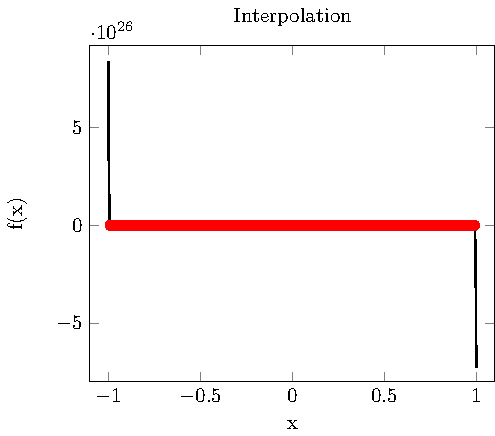
\includegraphics[width=0.4\textwidth]{./Uniform_100.pdf}
		}
		\subfigure[$200$ nodes]{
			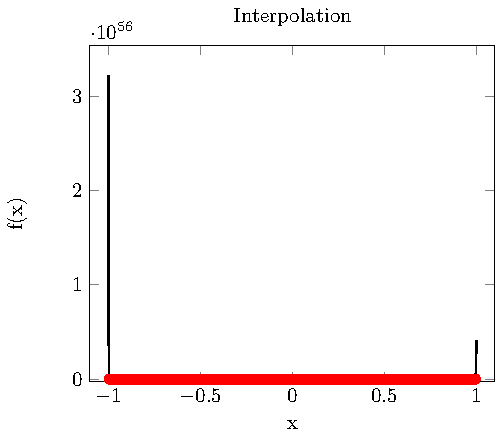
\includegraphics[width=0.4\textwidth]{./Uniform_200.pdf}
		}

		\caption{Interpolation with random data at Uniform nodes}
		\end{center}
	\end{figure}
	
	\begin{center}
		\Huge Chebyshev node interpolation
	\end{center}
	\begin{figure}[!htbp]
		\begin{center}
		\subfigure[$5$ nodes]{
			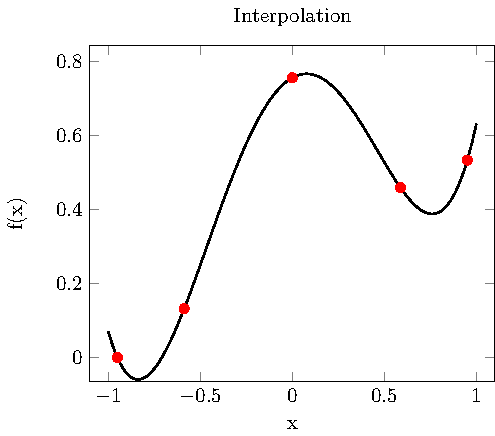
\includegraphics[width=0.4\textwidth]{./Chebyshev_5.pdf}
		}
		\subfigure[$10$ nodes]{
			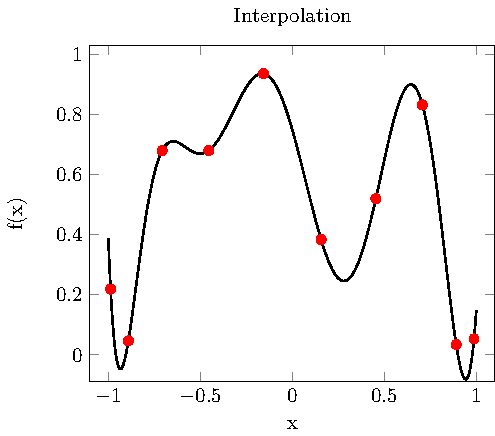
\includegraphics[width=0.4\textwidth]{./Chebyshev_10.pdf}
		}

		\subfigure[$20$ nodes]{
			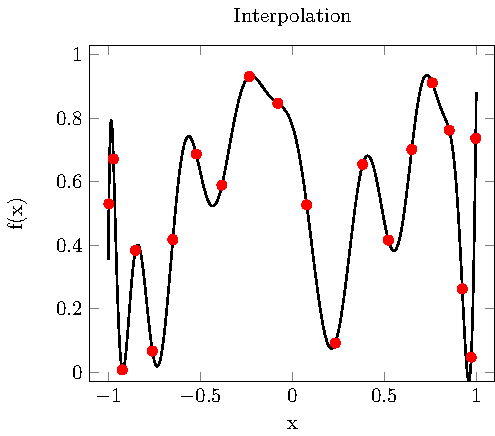
\includegraphics[width=0.4\textwidth]{./Chebyshev_20.pdf}
		}
		\subfigure[$50$ nodes]{
			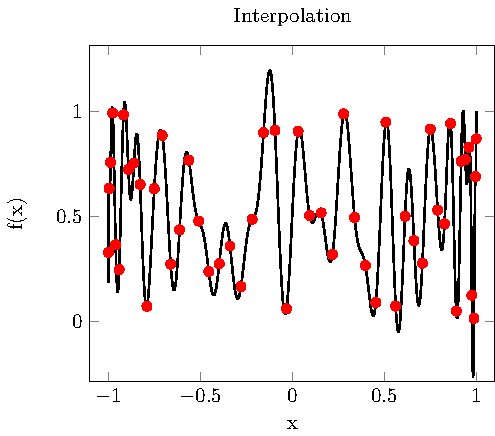
\includegraphics[width=0.4\textwidth]{./Chebyshev_50.pdf}
		}

		\subfigure[$100$ nodes]{
			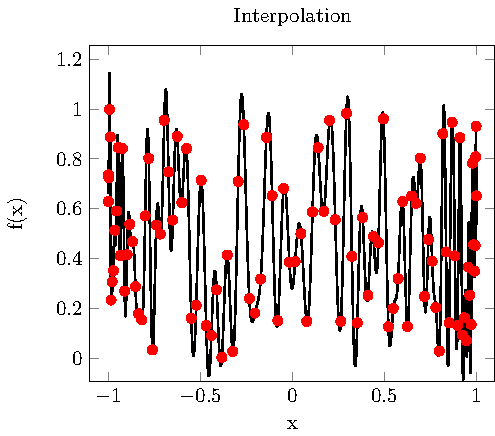
\includegraphics[width=0.4\textwidth]{./Chebyshev_100.pdf}
		}
		\subfigure[$200$ nodes]{
			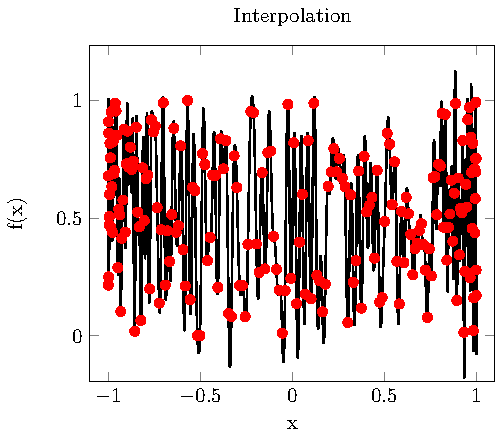
\includegraphics[width=0.4\textwidth]{./Chebyshev_200.pdf}
		}

		\caption{Interpolation with random data at Chebyshev nodes}
		\end{center}
	\end{figure}
\end{document}